\documentclass[a4paper, 12pt, final, garamond]{book}
\usepackage{cours-preambule}

\raggedbottom

\makeatletter
\renewcommand{\@chapapp}{M\'ecanique -- chapitre}
\makeatother

\begin{document}
\setcounter{chapter}{3}

\chapter{Correction TD application}
\section{Intérêt des raisonnements énergétiques}

\begin{enumerate}
    \item
        \begin{minipage}[t]{0.48\linewidth}
            À $t=0$, la balle est lancée en $z = 0$ avec une vitesse $\vfo =
            v_O\uz$. Elle va monter en altitude en perdant de l'énergie cinétique et
            en gagnant en énergie potentielle. \bigbreak
            Le système \{masse\} n'est soumis qu'au poids, qui est conservatif~; le
            système est donc conservatif et l'énergie mécanique se conserve~:
        \end{minipage}
        \hfill
        \begin{minipage}[t]{0.50\linewidth}
            ~
            \begin{center}
                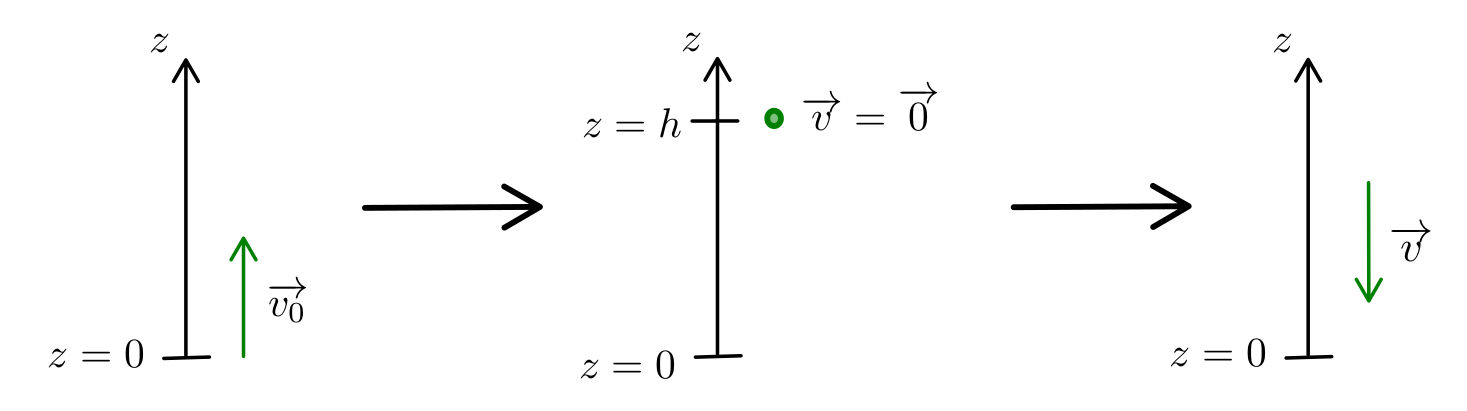
\includegraphics[width=\linewidth]{hmax_vert_corr}
                \captionof{figure}{Schéma de la situation}
                \label{fig:penduleztt}
            \end{center}
        \end{minipage} \bigbreak
        \[\dv{\Ec_m}{t} = 0\]
        Ainsi,\vspace*{-24pt}
        \begin{align*}
            \Ec_m(0) &= \Ec_m(t_{\max})
            \\\Lra
            \frac{1}{2}\cancel{m}v_0{}^2 + \underbracket{mgz_0}_{=0}
                     &=
            \frac{1}{2}\cancel{m}v(t_{\max})^2 + \cancel{m}gh
            \\\Lra
            \Aboxed{h &= \sqrt{\frac{v_0{}^2}{2g}}}
            \qed
        \end{align*}
    \item
        \begin{minipage}[t]{0.70\linewidth}
            Le système est conservatif puisque le poids est une force conservative
            et que le travail de la force de tension est nul ($\Tf \perp \vf$). On
            peut donc utiliser le TEM en déterminant l'énergie potentielle en
            fonction de $\tt$. \bigbreak
            On prend la référence d'altitude $z = 0$ en bas du pendule. La longueur
            du pendule étant $\ell$, on trouve l'altitude en projetant le point M
            sur l'axe $z$ pour trouver
        \end{minipage}
        \hfill
        \begin{minipage}[t]{0.28\linewidth}
            \vspace*{-1cm}
            \begin{center}
                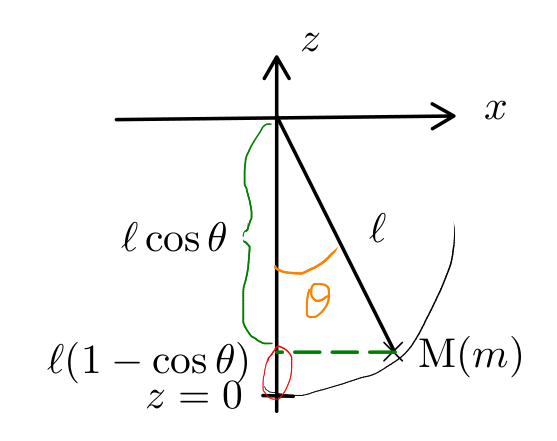
\includegraphics[width=\linewidth]{thetamax_pend_corr}
                \captionsetup{justification=centering}
                \captionof{figure}{Schéma pour $z(\tt)$}
                \label{fig:penduleztt}
            \end{center}
        \end{minipage}
        \[z(\tt) = \ell(1-\cos\tt)\]
        Ainsi,
        \begin{align*}
            \D_{\ABr}\Ec_m &=0
            \\\Lra
            \frac{1}{2}\cancel{m}v_0{}^2 + \underbracket{mgz_0}_{=0}
                     &=
            \frac{1}{2}\cancel{m}v_{\max}{}^2 + \cancel{m}gz_{\max}
            \\\Lra
            \ell(1-\cos\tt_{\max}) &= \frac{v_0{}^2}{2g}
            \\\Lra
            \Aboxed{\cos\tt_{\max} &= 1 - \frac{v_0{}^2}{2g\ell}}
            \qed
        \end{align*}
        Cette équation est valable si $v_0{}^2/2g\ell < 2$, sinon
        $\cos\tt_{\max} < -1$. Cette condition traduit le fait que le pendule ne
        fait pas des tours, i.e. ne dépasse pas $\tt = \pi$.
\end{enumerate}

\section{Curling}
\begin{enumerate}
    \item On a simplement
        \[
            \Ec_{c,I} = \frac{1}{2}mv_0{}^2
            \qet
            \Ec_{c,F} = 0
        \]
    \item 
        \begin{minipage}[t]{0.40\linewidth}
            \begin{itemize}[label=$\diamond$, leftmargin=10pt]
                \litem{Système~:} \{pierre\}
                \litem{Référentiel~:} $\Rc\ind{piste}$, galiléen
                \litem{Repère~:} $(\Or,\ux,\uz)$
                \litem{Repérage~:}
                    \begin{gather*}
                        \OM = x\ux\\
                        \vv{\rm OM_0} = D\ux\\
                        \vf = \xp\ux
                    \end{gather*}
            \end{itemize}
        \end{minipage}
        \hfill
        \begin{minipage}[t]{0.65\linewidth}
            ~
            \begin{center}
                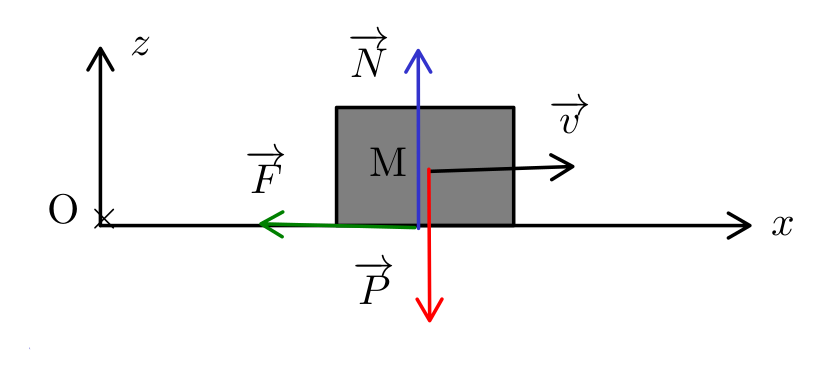
\includegraphics[width=.8\linewidth]{curling_corr}
                \captionof{figure}{Schéma de la situation}
                \label{fig:curling}
            \end{center}
        \end{minipage} \bigbreak
        \begin{itemize}[label=$\diamond$, leftmargin=10pt]
            \litem{BDF et BDW~:}
                \[
                    \begin{array}{ll}
                        \textbf{Poids} & \Pf = -mg\uz\\
                        \textbf{Réaction} & \Nf = N\uz\\
                        \textbf{Frottements} & \Ff = -F_0\ux
                    \end{array}
                    \quad\Ra\quad
                    \begin{array}{llll}
                        W_{\rm OM_0}(\Pf) &= \Pf\cdot\vv{\rm OM_0} &=
                        -mgD(\underbracket{\uz\cdot\ux}_{=0}) &= 0\\
                        W_{\rm OM_0}(\Nf) &= \Nf\cdot\vv{\rm OM_0} &=
                        ND(\underbracket{\uz\cdot\ux}_{=0}) &= 0\\
                        W_{\rm OM_0}(\Ff) &= \Ff\cdot\vv{\rm OM_0} &=
                        -F_0D(\underbracket{\ux\cdot\ux}_{=1}) &= -F_0D
                    \end{array}
                \]
        \end{itemize}
    \item Ici,\vspace*{-24pt}
        \begin{align*}
            \D_{\rm OM_0}\Ec_c &= \sum_i W_{\rm OM_0}(\Ff_i)
            \\\Lra
            0 - \frac{1}{2}mv_0{}^2 &= -F_0D
            \\\Lra
            \Aboxed{v_0 &= \sqrt{\frac{2F_0D}{m}}}
            \qed
            \qavec
            \left\{
                \begin{array}{rcl}
                    F_0 & = & \SI{3.0}{N}\\
                    D   & = & \SI{25}{m}\\
                    m   & = & \SI{20}{kg}
                \end{array}
            \right.\\
            \AN
            \Aboxed{v_0 &= \SI{2.7}{m.s^{-1}}}
        \end{align*}
\end{enumerate}

\section{Piégeage d'un électron}
\begin{enumerate}
    \item 
        \begin{minipage}[t]{0.30\linewidth}
            ~
            \begin{center}
                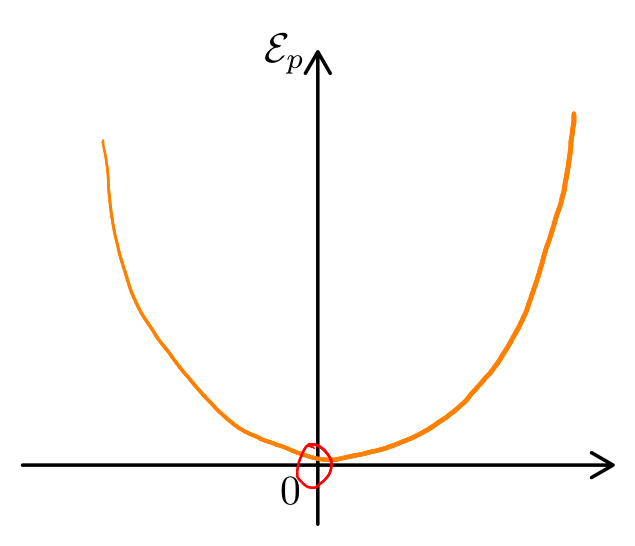
\includegraphics[width=\linewidth]{piege_elec_corr}
                \captionof{figure}{$\Ec_p(z)$}
                \label{fig:piegeelec}
            \end{center}
        \end{minipage}
        \hfill
        \begin{minipage}[t]{0.65\linewidth}
            On trace l'énergie potentielle, qui est \textbf{évidemment} une
            parabole convexe. On trouve le point d'équilibre en calculant sa
            dérivée et en trouvant quand elle s'annule~; visuellement, la
            dérivée s'annule en $z_{\eq} = 0$, mathématiquement
            \[\eval{\dv{\Ec_p}{z}}_{z_{\eq}} = \frac{eV_0}{d^2}z_{\eq} = 0 \Lra
            \boxed{z_{\eq} = 0}\]
            On trouve sa stabilité en évaluant sa dérivée seconde en ce point,
            et il sera stable si elle est positive. En tant que fonction convexe
            en ce point, il est visiblement stable. On calcule~:
        \end{minipage}
        \[\boxed{\eval{\dv[2]{\Ec_p}{z}}_{z_{\eq}} = \frac{eV_0}{d^2} > 0}\]
        Il est donc bien stable.
    \item Tout système conservatif autour de son point d'équilibre stable est
        régit par une équation d'oscillateur harmonique, faisant donc apparaître
        la pulsation propre $\w_0$. Il suffit pour démontrer cela d'utiliser la
        caractéristique principale d'un système conservatif~: le fait que son
        énergie mécanique se conserve, i.e. $\dv{\Ec_m}{t} = 0$. En effet, le
        TPC nous indique
        \[\dv{\Ec_m}{t} = \sum_i \underbracket[1pt][.8em]{\Pc(\Ff_{{\rm
        NC},i})}_{\mathclap{=0\text{ car conservatif}}} = 0\]
        On nous donne $\Ec_p(z)$, donc pour avoir $\Ec_m$ il faut trouver la
        vitesse de la particule. Rien n'est indiqué dans l'énoncé, mais le
        problème n'indique qu'un potentiel selon $\uz$~; on peut supposer que la
        vitesse ne se fait que selon $\uz$ également, et qu'on a donc $\vf =
        \zp\uz$. Ainsi,
        \begin{align*}
            \dv{\Ec_m}{t} &= 0
            \\\Lra
            \dv{t}(\Ec_c + \Ec_p) &= 0
            \\\Lra
            \dv{t}(\frac{1}{2}m\zp^2 + \frac{eV_0}{2d^2}z^2) &= 0
            \\\Lra
            m\cancel{\zp}\zpp + \frac{eV_0}{d^2}z\cancel{\zp} &= 0
            \\\Lra
            \Aboxed{\zpp + \w_0{}^2z &= 0}
            \qavec
            \boxed{\w_0 = \sqrt{\frac{eV_0}{md^2}}}
        \end{align*}
        Étant donné que $\w_0 = 2\pi f_0$, on obtient finalement
        \begin{align*}
            \Aboxed{f_0 &= \frac{1}{2\pi}\sqrt{\frac{eV_0}{md^2}}}
            \qed
            \qavec
            \left\{
                \begin{array}{rcl}
                    e   & = & \SI{1.6e-19}{C}\\
                    V_0 & = & \SI{5.0}{V}\\
                    m   & = & \SI{9.1e-31}{kg}\\
                    d   & = & \SI{6.0e-3}{m}
                \end{array}
            \right.\\
            \AN
            \Aboxed{f_0 &= \SI{25}{MHz}}
        \end{align*}
    \item Une force conservative dérive d'une énergie potentielle selon
        \begin{align*}
            \Ff &= -\gd\Ec_p
            \\\Lra
            \Ff &=
            -\mqty(\DS\pdv{\Ec_p}{x}\\[1em]\DS\pdv{\Ec_p}{y}\\[1em]\DS\pdv{\Ec_p}{z})
            =
            -\mqty(0\\0\\\DS\frac{eV_0}{d^2}z)
            \\\Lra
            \Aboxed{\Ff &= - \frac{eV_0}{d^2}z\uz}
            \qed
        \end{align*}
\end{enumerate}

\section{Balle dans un tonneau}
\begin{enumerate}
    \item 
        \begin{minipage}[t]{0.65\linewidth}
            \begin{itemize}[label=$\diamond$, leftmargin=10pt]
                \litem{Système~:} \{balle\}
                \litem{Référentiel~:} $\Rc\ind{sol}$, supposé galiléen
                \litem{Repère~:} cartésien pour la chute sur la rampe, avec $\uz$
                    vertical ascendant, et $({\rm C}, \ur, \ut)$ quand la balle est
                    dans le tonneau~; voir schéma
                \litem{Repérage~:} dans le tonneau,
                    \begin{align*}
                        \vv{\rm CM} &= R\ur\\
                        \vf_{\Mr} &= R\tp\ut\\
                        \af_{\Mr} &= R\tpp\ut -R\tp^2\ur
                    \end{align*}
            \end{itemize}
        \end{minipage}
        \hfill
        \begin{minipage}[t]{0.30\linewidth}
            ~
            \begin{center}
                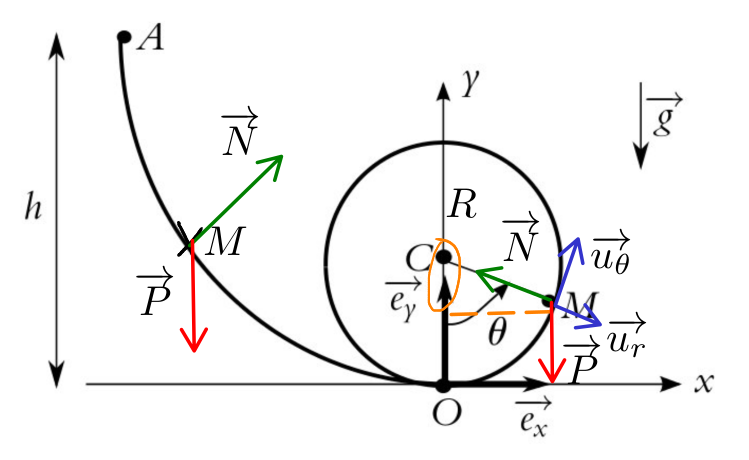
\includegraphics[width=\linewidth]{tonneau_corr}
                \captionsetup{justification=centering}
                \captionof{figure}{Schéma de la situation}
                \label{fig:tonneau_corr}
            \end{center}
        \end{minipage}
        \begin{itemize}[label=$\diamond$, leftmargin=10pt]
            \litem{BDF~:} dans le tonneau,
                \[
                    \begin{array}{ll}
                        \textbf{Poids} & \Pf = mg(\cos\tt\ur-\sin\tt\ut)\\
                        \textbf{Réaction} & \Nf = -N\ur
                    \end{array}
                \]
            \litem{BDW~:}
                \begin{align*}
                    W_{\rm AM}(\Nf) &= 0 \quad (\Nf\perp\dd\OM)\\
                    \Pf &= \text{conservatif}
                \end{align*}
                Le système est donc \textbf{conservatif}. On peut appliquer le
                TEM~:
            \litem{En A~:} $v_\Ar = 0$, $z_\Ar = h$
            \litem{En O~:} $v_\Or = v_\Or$, $\boxed{z_\Or = 0} \Leftarrow$ référence
                \textbf{pour toute l'étude}
            \litem{En M~:} $z(\tt) = R(1-\cos\tt)$
            \litem{TEM~:}
                \begin{align*}
                    \D_{\rm AO}\Ec_m &= 0
                    \\\Lra
                    \cancel{m}gh &= \frac{1}{2}\cancel{m}v_\Or{}^2
                    \\\Lra
                    \Aboxed{v_\Or &= \sqrt{2gh}}
                    \qed
                    \shortintertext{Puis}
                    \D_{\rm OM}\Ec_m &= 0
                    \\\Lra
                    \xoverbracket{\frac{1}{2}\cancel{m}v_\Mr{}^2}^{\Ec_c(\Mr)} +
                    \xoverbracket{\cancel{m}gR(1-\cos\tt)}^{\Ec_{p,p}(\Mr)}
                                     &=
                    \xoverbracket{\frac{1}{2}\cancel{m}v_\Or{}^2}^{\Ec_c(\Or)} +
                    \xoverbracket{\xunderbracket{mgz_\Or}_{=0}}^{\Ec_{p,p}(\Or)}
                    \\\Lra
                    v_\Mr &= \sqrt{v_\Or{}^2 + 2gR(\cos\tt-1)}
                    \\\Lra
                    \Aboxed{v_\Mr &= \sqrt{2g}\sqrt{h + R(\cos\tt-1)}} = R\tp
                    \qed
                \end{align*}
        \end{itemize}
    \item On sort de l'analyse énergétique, puisqu'on veut une valeur de force
        \textbf{en un point} du mouvement. On applique donc le \textbf{PFD}~:
        \begin{align*}
            m\af &= \Pf + \Nf
            \\\Lra
            \left\{
                \begin{aligned}
                    -mR\tp^2 &= mg\cos\tt-N\\
                    mR\tpp &= -mg\sin\tt
                \end{aligned}
            \right.
                 &\Ra
            N = mg\cos\tt + mR\tp^2
        \end{align*}
        Or, $v_\Mr = R\tp \Lra v_\Mr{}^2 = R^2\tp^2 \Lra R\tp^2 = v_\Mr{}^2/R$
        donc
        \begin{align*}
            N &= m\left(g\cos\tt + \frac{2g}{R}\left(h+R(\cos\tt-1)\right)\right)
            \\\Lra
            N &= m\left(g\cos\tt + 2g\cos\tt -2g + 2g \frac{h}{R}\right)
            \\\Lra
            \Aboxed{N &= mg\left(3\cos\tt - 2 + 2 \frac{h}{R}\right)}
            \qed
        \end{align*}
    \item La condition de contact entre deux solides est que la réaction normale
        ne soit pas nulle. Autrement dit, si la réaction normale est nulle, il
        n'y a plus contact~: on cherche donc ici à voir si $N > 0$ à chaque
        instant. On pourrait tracer la fonction $N(\tt)$, mais on remarque
        facilement que l'endroit où $N$ est la plus susceptible de s'annuler est
        quand $\tt = \pi$, quand la belle est «~la tête à l'envers~». On résout
        donc
        \begin{align*}
            N(\pi) &> 0
            \\\Lra
            \cancel{mg}\left(-3-2+2\frac{g}{R}\right) &> 0
            \\\Lra
            2\frac{h}{R} &> 5
            \\\Lra
            \Aboxed{h &> \frac{5}{2}R} = h_{\min}
            \qed
        \end{align*}
\end{enumerate}

\end{document}
